\chapter{Realisation of a demonstrator}
%\textbf{keep it small and simple} 
%Outline of the technologies used to fabricate and assemble your structures, if applicable. Detailed processes belong in the appendix. If numerous types of structures were fabricated, or assembly technology is extensive, there may be more than one of these chapters. \textbf{Characterization} Description of the means developed and employed to characterize the devices or systems that have been fabricated.
%The realisation of the demonstrated concepts on a hybrid substrate was one goal of this thesis, to show its feasibility.
The demonstrators realized in this work consisted of several \gls{ab:mmic} chips with a filter network built by discrete elements.
Due to the fact that \gls{ab:smd} decoupling capacitors as well as \gls{ab:mmic} were used, this were called hybrid test circuit.
%In fact of the combination of \gls{ab:mmic} and the discrete components the demonstrator described a hybrid test circuit.
% Therefore the realised demonstrator is a hybrid test circuit.
For assembling and measurement purposes the test circuit was restricted to a resolution of two bit.
Otherwise the bonding, assembling and controlling of the inputs would became too complex.
% To avoid building a too complex structure the resolution of the \gls{ab:dac} was restricted to two bit.
Two bit resolution implied to create an input control strategy for the four inputs.
A third bit of resolution would enhance the performance but also increase the complexity of the realisation as six inputs needed to e controlled.
% As well the bonding of the chips, the heat transfer, power consumption
%If a third bit of resolution was added this would increase the number of inputs to six, which makes the circuit and the test setup more complex.
\\
A two layer high frequency substrate, namely Rogers RO4003, were used.
The benefit of the low dissipation factor, a low tolerance of dielectric coefficient and the stable electrical properties made this the most suitable material for the broadband application. %ref-> datasheet???

%Low dielectric tolerance, low loss, stable electrical properties and low thermal coefficient made this substrate the most suitable for the desired application.
%The benefit of this substrate were excellent electrical performance which made it ideal for broadband applications.
%The dissipation factor is 0.0027, while dielectric constant is 3.55 and thermal coefficient is +40. % which parameters are really helpfull in contrast to other materials?
With the help of former designed chips, two different versions of the substrate were designed.
To made use of these chips it was necessary to design two different versions due to the different properties of the chips.
% created at the IAF by Stephan Maroldt. % name it here? reference to a paper or a design process?
The two layer substrates were ordered with a thickness of \SI{0.508}{\milli \metre}, a \SI{35}{\micro \metre} \gls{ab:cu} conduction layer and a \gls{ab:ChemNiPdAu} metallisation.
An impedance control ensured the correct impedance of \SI{50}{\ohm} for the \SI{1.1}{\milli \meter} wide \gls{ab:msl} at the in- and output of the circuit.

% of the \SI{50}{\ohm} input lines as well for the \SI{50}{\ohm} output line is performed by the manufacturer, Contag AG, to ensure the best matching.

Each version of the designed substrates had the size of \SI{60}{\milli \meter} x \SI{54}{\milli \meter} while the area for the multi assembled chips covered approximately \SI{6}{\milli \meter} x \SI{5.5}{\milli \meter} for both.
% The different version are designed with the background of using different chips with different properties.
One layout was designed for chips which ground contact were plated through the backside metallization of the chip.
Yielding a power transistors source contact connected to these ground plates.
This property yielded a great drawback compared to the other layout.\\
The second layout of the substrate were planned to improve the heat transfer by using another type of chip.
This chips ground contact were not plated through the backside metallization, making them suitable for soldering on a conducting heat spreader.\\
%The designed schematic needed a power transistor which switched the power supply voltage to the output of the circuit.
%For this functionality the transistors source contact acted like the output and therefore it should not be connected to ground potential.
%Therefore this version could be mounted (soldered) to the conduction layer without the need of an isolated pad.
%These chips DDRi\_2C, also designed by Stephan Maroldt, have to be bonded to the substrate GND separately.
To made use of the former designed chips, these two layouts were designed to enable the proof of concept.


\section{Substrate layout using DDRi\_X6 and DDRi\_Y6 chips}
%\begin{enumerate}
%	\item Highside driver load transistor voltage connected to Vdd
%	\item Highside driver load transistor voltage connected to Vout
%\end{enumerate}

The presented layout of the substrate was designed for the use of the chips DDRi\_X6 and DDRi\_Y6 since the chip DDRi\_2C required a different multi chip connection.
Figure \ref{fig:layoutDDRiXY6sub} shows the overview of the designed substrate, consisting of a decoupling capacitor network, several dc voltage and \gls{ab:rf} connectors and the core of the circuit.

\begin{figure}[htb!]
	\centering
  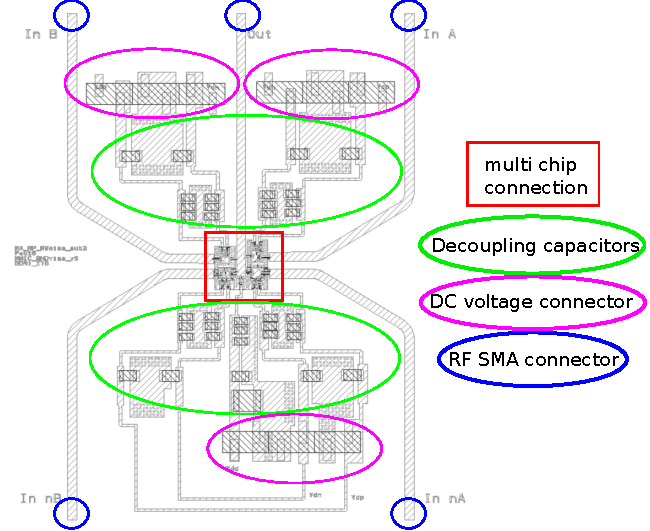
\includegraphics{Layout_DDRiXY6_new_grey.pdf}
	\caption{Layout substrate with DDRi\_XY6 chips}
	\label{fig:layoutDDRiXY6sub}
\end{figure}

%To realize a high side switch with those chips, they have to be put on a pad without gnd contact.
%The source contact of the chip is the output for the high side, while the source contact of the lowside switch is grounded.
%Therefore for the lowside the chips is mounted on the ground layer.
%Chips with this properties are designed by Stephan Maroldt, namely DDRi\_X6 and DDRi\_Y6.

It is to mention that the layout outside the red marked box was very similar for the others version.
So one explanation of the layout outside the box were sufficient.
Only one additional \gls{ab:dc} voltage supply line was added and the arrangement of the chips were different.
Due to the different arrangement of the chips attention was paid to the connection of bias voltages.\\
The described part outside the red box consists of the \gls{ab:smd} decoupling capacitor filter network and the multi pin connector for the \gls{ab:dc} voltage supply.
In addition to this the in- and output transmission lines were designed to fit to an \SI{50}{\ohm} impedance. \\
The decoupling capacitors, also known as bypass capacitors, filtered out undesired frequency portions by the power supply.
If the filter network did not work properly, this could lead to undesired oscillations of the circuit.
Following a very common design rule lead to the right choice of capacitors.
A very first decoupling capacitor was integrated on the \gls{ab:mmic} chip.
The requirement to place the decoupling capacitors as close as possible to the \gls{ab:dc} voltage supply pad lead to the choice of a special \gls{ab:mmic} capacitor.
It was possible to place that capacitor as near as possible to the chip to keep the length of the bonds small.
To avoid resonance peaking the most suitable capacitors were those with a high \gls{ab:esr} since the quality factor of these were small.
A great bypassing range were enabled by choosing a \SI{82}{\pico \farad} capacitor, namely D20BT820K5PX from Dielectric Laboratories Inc., to filter out frequencies in the GHz range.
The gold metallization (for wire bonding), the thin film technology and the custom sizes (to keep it small), made this the most suitable capacitor for the purpose filtering high frequencies.
Each capacity, of subsequent capacitors, were increased by one order in magnitude yielding the biggest capacity of \SI{10}{\micro \farad}.
The big capacity filtered out frequency portions in the lower kHZ range.
% Reference !! -> decoup. bypass cap paper
% literature on this topic !! -> explain the choice of capacitor size !!!
In addition to the capacity also the temperature and voltage range had to fit.
%(Bypassing and operating frequency not necessarily linked to each other. Bypassing a greater range than the potential operating frequency)
% (Culture Cargo principle). 
The following choice for the capacities was taken: \SI{82}{\pico \farad}, \SI{1}{\nano \farad}, \SI{10}{\nano \farad}, \SI{100}{\nano \farad}, \SI{1}{\micro \farad}, \SI{10}{\micro \farad}, started at the chips supply pin. \\
In fact that oscillation still could appear, the size of the used pads was designed larger, making it possible to change (adapt) the capacities for the filter network.
These pads also had some via holes to transfer the ambient temperature to the backside.
This was the attempt to keep as much as possible heat away from the chips.\\
The four input lines, as well as the output line, were designed to fit to an impedance of \SI{50}{\ohm}.
With a line calculator, namely line calc in the program ads, the corresponding line width was calculated.
The calculated width of the line was \SI{1.1}{\milli \meter} which was checked by the manufacturer with an impedance control as well.\\
The arrangement of the chips was realised to keep the length of the bond wires as short as possible.
However the distances between conduction lines were limited by the process of the manufacturer.
The transmission lines of the signal path were designed to fit each other.
All transmission lines were matched to \SI{50}{\ohm} and got the same length to avoid undesired delays of the signal.
An important fact to consider was that all switches had to switch synchronous at the same time. 
Therefore no signal delays were permitted, induced by different transmission lines.\\
The assembly of the multi chip connection marked with the red rectangular is described in Figure \ref{fig:layoutDDRiXY6bond}.

\begin{figure}[htb!]
	\centering
  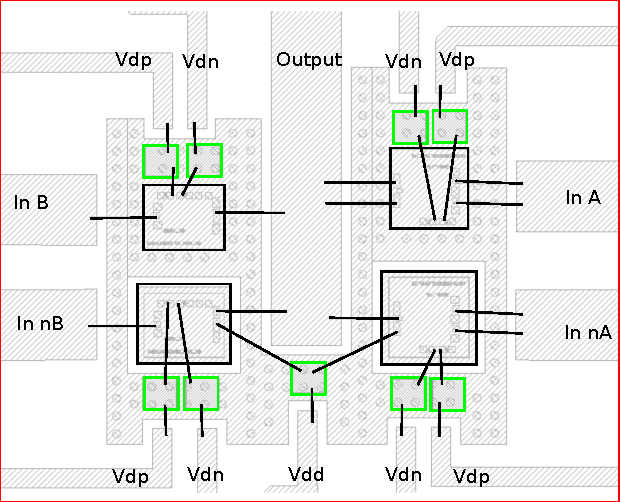
\includegraphics{Layout_DDRiXY6_bonds_new.pdf}
	\caption{Layout DDRi\_X6 and DDRi\_Y6 chips}
	\label{fig:layoutDDRiXY6bond}
\end{figure}

%One very important design rule for this layout was to create as much as possible heat transfer.
The drawback of these chosen chips were its plated through ground contact. 
In fact of this, a proper function of these chips as a high side switch, made it necessary to place it on an electrical isolated pad.
At the bottom of Figure \ref{fig:layoutDDRiXY6bond} these chips were placed on an isolated pad.
This pad did not have any connection to the backside potential of the substrate.
The pads were surrounded by a large conducting layer with via holes to spread the heat.
The idea was to dissipate the heat over the air bridge, through the via holes of the conducting layer, to the backside of the substrate.
%This was not the optimal but a cost effective way to dissipate the heat.
%A more expensive way would be to take a ceramic for the isolation.
The substrate was mounted on a beam(?), which improved the cooling a little bit.
The beam was necessary to install the RF-SMA connectors and therefore the connection between the circuit and the measurement equipment.
This was a very critical design issue since the chips created much power, hence much heat.
\\
As mentioned earlier the length of the bond wires were set to be equal for the signal paths.
Since an in-phase control of the input was important to ensure the switches to turn on/off synchronous.
The length of the bond wires providing the \gls{ab:dc} voltage supply were not critical.
The diameter of the wedged \gls{ab:au} bond wires was set to \SI{25}{\micro \metre} which ensured a maximum current of approximated \SI{1}{\ampere} for a bond length of \SI{1}{\milli \metre}.
The small diameter and the short length made it most suitable for the high frequency application.\\
Figure \ref{fig:photoDDRiXY6bond} shows the assembling of the used chips with their corresponding bond wires.
As mentioned the bond wires got the same length for the signal path.


\begin{figure}[htb!] %% DRucken pddf verwenden
	\centering
  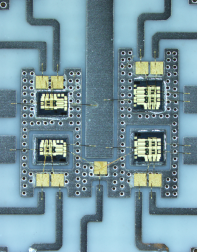
\includegraphics{Photo_DDRi_XY6.png}
	\caption{Photograph of assembled DDRi\_X6 \& DDRi\_Y6 chips}
	\label{fig:photoDDRiXY6bond}
\end{figure}

%########################## important stability factor !!! ########################
%A positive feedback of the used amplifiers had to be avoided.
%To eliminate undesirable feedback the driver circuit had to be assembled without feedback path.

%%%%%%%%%%%%%%%%%%%%%%%%%13.04.2016; 20:06 Uhr %%%%%%%%%%%%%%
\newpage
\section{Substrate layout using DDRi\_2C chips}
The layout of the filter network and the \gls{ab:dc} supply voltage did not differ as much from the previous presented layout version.
In this second layout one additional \gls{ab:dc} connector was added and the arrangement of the chips differed.
Figure \ref{fig:layoutDDRi2Cbond} shows the arrangement of the used chips, namely DDRi\_2C.


\begin{figure}[htb!]
	\centering
  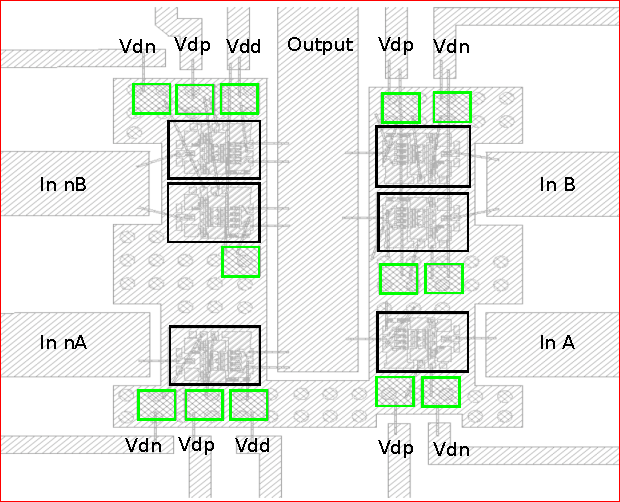
\includegraphics{Layout_DDRi2C_bonds.pdf}
	\caption{Layout DDRi\_2C chips}
	\label{fig:layoutDDRi2Cbond}
\end{figure}

Due to the fact that six chips were used in this layout, the wiring of bonds was more complex.
Also the placement of the high and low side switches differed in contrast to the previous layout.
The switches, representing one bit of resolution, were placed horizontally while the previous layout showed the switches placed vertically.
Horizontal alignment was chosen due to easier bond wiring.
This led to a different bias voltage connections.\\

The most important difference in the two layouts were the difference of used chips.
The chips used in this layout version, DDRi\_2C chips did not have a plated through hole to its backside.
Thus, these chips could be soldered directly to the heat spreading backside connected layer.
The heat could transfer directly from the backside of the chip through the via holes to the substrates backside.
This improved the heat transfer a lot in contrast to the first design.
It must be pointed out to connect the ground potential of the chips separately to the boards ground potential.
This version might work better due to the better heat dissipation, although the fabrication of the chips was older (2011).\\
The assembled chips for the second version is shown in Figure \ref{fig:photoDDRi2Cbond}.

\begin{figure}[htb!] %% Drucken pdf verwenden!
	\centering
  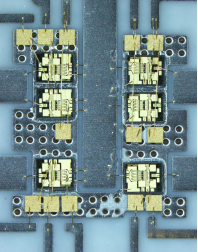
\includegraphics{Photo_DDRi_2C.png}
	\caption{Photograph of assembled DDRi\_2C chips}
	\label{fig:photoDDRi2Cbond}
\end{figure}

% Problem of BANDWIDTH, Vpp of control signal (5V pp for GaN transistors), high side driver, 
%Control voltage of 5 V realization with OPAMPS? Possible to overdrive opamps instead of using broadband ppa.
\section{Evaluation of the design and realisation process}
After simulating the theoretical concept, in the realisation process a great number of aspects had to be considered.
Since it was the first time ever to built this concrete test circuit with \gls{ab:gan} technology, no validated concepts could be used.
In the following the most crucial aspects are described.
The circuit was built on a hybrid assembly which combines the \gls{ab:mmic} with the discrete \gls{ab:smd} components on a Rogers 4003 substrate.
The input and output lines on the substrate were \gls{ab:msl} which were matched to \SI{50}{\ohm}.
Important for the design of the input lines were that they are of the same length, due to timing issues.
In addition to this, rectangular edges were avoided to reduce parasitic effects.
The input timing is crucial due to the fact that the switches have to switch synchronous.
The output line was matched to \SI{50}{\ohm} to ensure proper measuring.
In addition to the same length of the input lines, also the bond wires of the in- and output to the \gls{ab:mmic} chips had to be of the same length.
One of the most important and crucial things was the dissipation of heat.
Based on the designed chips, two different concepts were realized to handle the dissipation of heat in the most proper way.
The wafer run of the chips DDRi\_2C was from the year 2011 and therefore five years old and hence the taping of the wafer could not be as good as the newer ones DDRi\_X6 and DDRi\_Y6.
Due to this heat dissipation problem it was renounced to package the chips into a \gls{ab:qfn} package.
\SI{25}{\micro \metre} (diameter) \gls{ab:au} bonds were used where the length of the bonds were given by assembly limits for spacing of conducting layers due to manufacturer process limits.
The minimum required number of bonds were used to avoid unnecessary parasitic inductances. 
But it is to mention that the huge amount of via holes, which were necessary to dissipate the heat, induces parasitic inductances.
In- and output connectors were commercially available \gls{ab:sma} jack connectors with a matched impedance of \SI{50}{\ohm} to connect standard RF cables.\\
The two layouts were fabricated by CONTAG AG while the used discrete components were ordered at Digi-Key Electronics.
The finished demonstrator is shown in Figure \ref{fig:assembledDemonstrator}with a short description of the placed elements.

\begin{figure}[htb!] %% zum drucken pdf verwenden
	\centering
  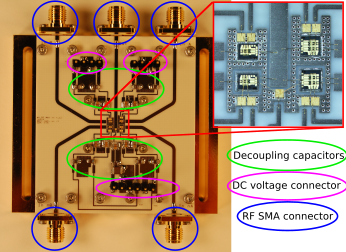
\includegraphics{Demonstrator_edited_newScale.png}
	\caption{Assembled demonstrator}
	\label{fig:assembledDemonstrator}
\end{figure}

\newpage
An improvement for the layout, could be to solder the DDRi\_XY6 chips on an electrical insulator while thermal good conductor, as AluminiumNitrid (AlN: 180-200 W/mK). 
This is needed to ensure the isolation from the output port to ground potential, but still have a good thermal transfer.
This pads would have needed a proper adhesive or solder which exhibit the same properties.
The desired pads would have been cut in very precise shapes and sizes, since the size of the chips DDRi\_X6 and DDRi\_Y6 were \SI{1.25}{\milli \meter} x \SI{1}{\milli \meter} and \SI{1.25}{\milli \meter} x \SI{1.25}{\milli \meter}, respectively.
This special material would have to be ordered and custom processed, while the performance when implemented in this concept, were not verified.
In fact of the special requirement, to order very small amount of the material which had to be cut in very precise pieces it was omitted to implement.
To test a first prototype the demonstrated concepts were sufficient.


\begin{figure}[htb!]
	\centering
  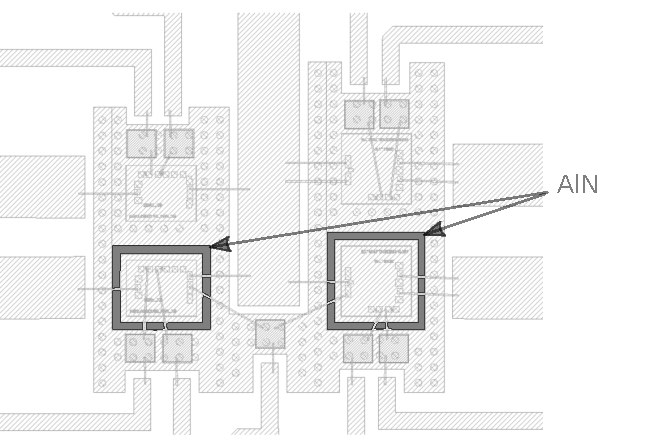
\includegraphics{Layout_DDRiXY6_AlN_pads.pdf}
	\caption{Improved layout for Chips DDRi\_X6 and DDRi\_Y6}
	\label{fig:DDRiXY6AlNpads}
\end{figure}